% shared preamble of the theory figures (white background, purple / black theme, sans-serif)
\documentclass[tikz,border=8pt]{standalone}
\usepackage[T1]{fontenc}
\usepackage[scaled=0.92]{helvet}
\renewcommand{\familydefault}{\sfdefault}
\usepackage{amsmath,amssymb}
\usepackage[helvet]{sfmath}
\usetikzlibrary{arrows.meta,calc,decorations.pathreplacing,positioning,backgrounds}
\definecolor{ink}{HTML}{1A1A1F}
\definecolor{cohesin}{HTML}{6A3DE8}
\definecolor{condensin}{HTML}{1BAF7A}
\definecolor{fwd}{HTML}{D1303F}      % CTCF pointing right
\definecolor{rev}{HTML}{2B62D9}      % CTCF pointing left
\definecolor{panel}{HTML}{F8F6FD}
\definecolor{panelline}{HTML}{E3DDF5}
\tikzset{
  fiber/.style={line width=2.1pt,ink,line cap=round,line join=round},
  halo/.style={line width=6pt,white,line cap=round},
  lab/.style={font=\small,text=ink},
  note/.style={font=\footnotesize,text=ink!60},
  hd/.style={font=\bfseries\small,text=ink,anchor=west},
  leader/.style={line width=0.6pt,ink!45},
}
% soft panel, numbered badge, heading
\newcommand{\panelbg}[4]{\draw[rounded corners=9pt,fill=panel,draw=panelline,line width=0.9pt] (#1,#2) rectangle (#3,#4);}
\newcommand{\badge}[3]{\fill[ink] (#1,#2) circle (0.21);\node[white,font=\bfseries\footnotesize] at (#1,#2) {#3};}
% CTCF: a protein on the fibre carrying an arrow that gives the motif direction (f = right, r = left)
\newcommand{\protf}[2]{\draw[rounded corners=3.5pt,line width=0.6pt,draw=fwd!65!black,fill=fwd] (#1-0.3,#2-0.19) rectangle (#1+0.3,#2+0.19);
  \draw[white,line width=1.5pt,-{Stealth[length=3.4pt,width=4.4pt]}] (#1-0.15,#2)--(#1+0.16,#2);}
\newcommand{\protr}[2]{\draw[rounded corners=3.5pt,line width=0.6pt,draw=rev!65!black,fill=rev] (#1-0.3,#2-0.19) rectangle (#1+0.3,#2+0.19);
  \draw[white,line width=1.5pt,-{Stealth[length=3.4pt,width=4.4pt]}] (#1+0.15,#2)--(#1-0.16,#2);}
\newcommand{\prot}[3]{\csname prot#3\endcsname{#1}{#2}}
% ring seen at an angle, drawn as a tube (dark outline, light core); back half and front half
\newcommand{\ringpart}[5]{\draw[line width=4.6pt,#3!80!black,line cap=round] ([shift={(#1,#2)}]#4:0.55 and 0.21) arc[start angle=#4,end angle=#5,x radius=0.55,y radius=0.21];
  \draw[line width=2.4pt,#3!55!white,line cap=round] ([shift={(#1,#2)}]#4:0.55 and 0.21) arc[start angle=#4,end angle=#5,x radius=0.55,y radius=0.21];}
\newcommand{\ringback}[3]{\ringpart{#1}{#2}{#3}{180}{0}}
\newcommand{\ringfront}[3]{\ringpart{#1}{#2}{#3}{180}{360}}
% smooth loop whose foot (ring) is at (cx,y0): half-width W, height H, ring colour
\newcommand{\lloop}[5]{%
  \ringback{#1}{#2}{#5}%
  \draw[fiber] (#1-0.3,#2) .. controls (#1-0.3,#2+0.25*#4) and (#1-#3,#2+0.2*#4) .. (#1-#3,#2+0.55*#4)
     .. controls (#1-#3,#2+0.95*#4) and (#1-0.5*#3,#2+#4) .. (#1,#2+#4)
     .. controls (#1+0.5*#3,#2+#4) and (#1+#3,#2+0.95*#4) .. (#1+#3,#2+0.55*#4)
     .. controls (#1+#3,#2+0.2*#4) and (#1+0.3,#2+0.25*#4) .. (#1+0.3,#2);%
  \ringfront{#1}{#2}{#5}}
% gently undulating fibre from x0 to the loop foot at cx (height y0), and from x1
\newcommand{\base}[4]{%
  \draw[fiber] plot[smooth] coordinates {(#1,0.05) (#1+0.35*#3-0.35*#1,-0.05) (#3-1.4,0.04)} .. controls (#3-0.6,0.02) and (#3-0.3,0.05) .. (#3-0.3,#4);
  \draw[fiber] plot[smooth] coordinates {(#2,-0.05) (#2-0.35*#2+0.35*#3,0.05) (#3+1.4,-0.04)} .. controls (#3+0.6,-0.02) and (#3+0.3,0.05) .. (#3+0.3,#4);}
% stop sign for a blocked leg and a leg arrow
\newcommand{\stopbar}[3]{\draw[#3,line width=2.4pt,line cap=round] (#1,#2-0.2)--(#1,#2+0.2);}
\newcommand{\legarrow}[3]{\draw[cohesin,line width=1.6pt,-{Stealth[length=5pt,width=6pt]},line cap=round] (#1,#3)--(#2,#3);}

\begin{document}
% \stage{x}{y}{W}{H}{d}: panel at (x,y) of width 8: fibre, loop (W x H) and CTCF at distance d from the ring
\newcommand{\stage}[5]{\begin{scope}[shift={(#1,#2)}]
  \base{0.4}{7.6}{4}{0.5}\lloop{4}{0.5}{#3}{#4}{cohesin}\prot{4-#5}{0}{f}\prot{4+#5}{0}{r}\end{scope}}
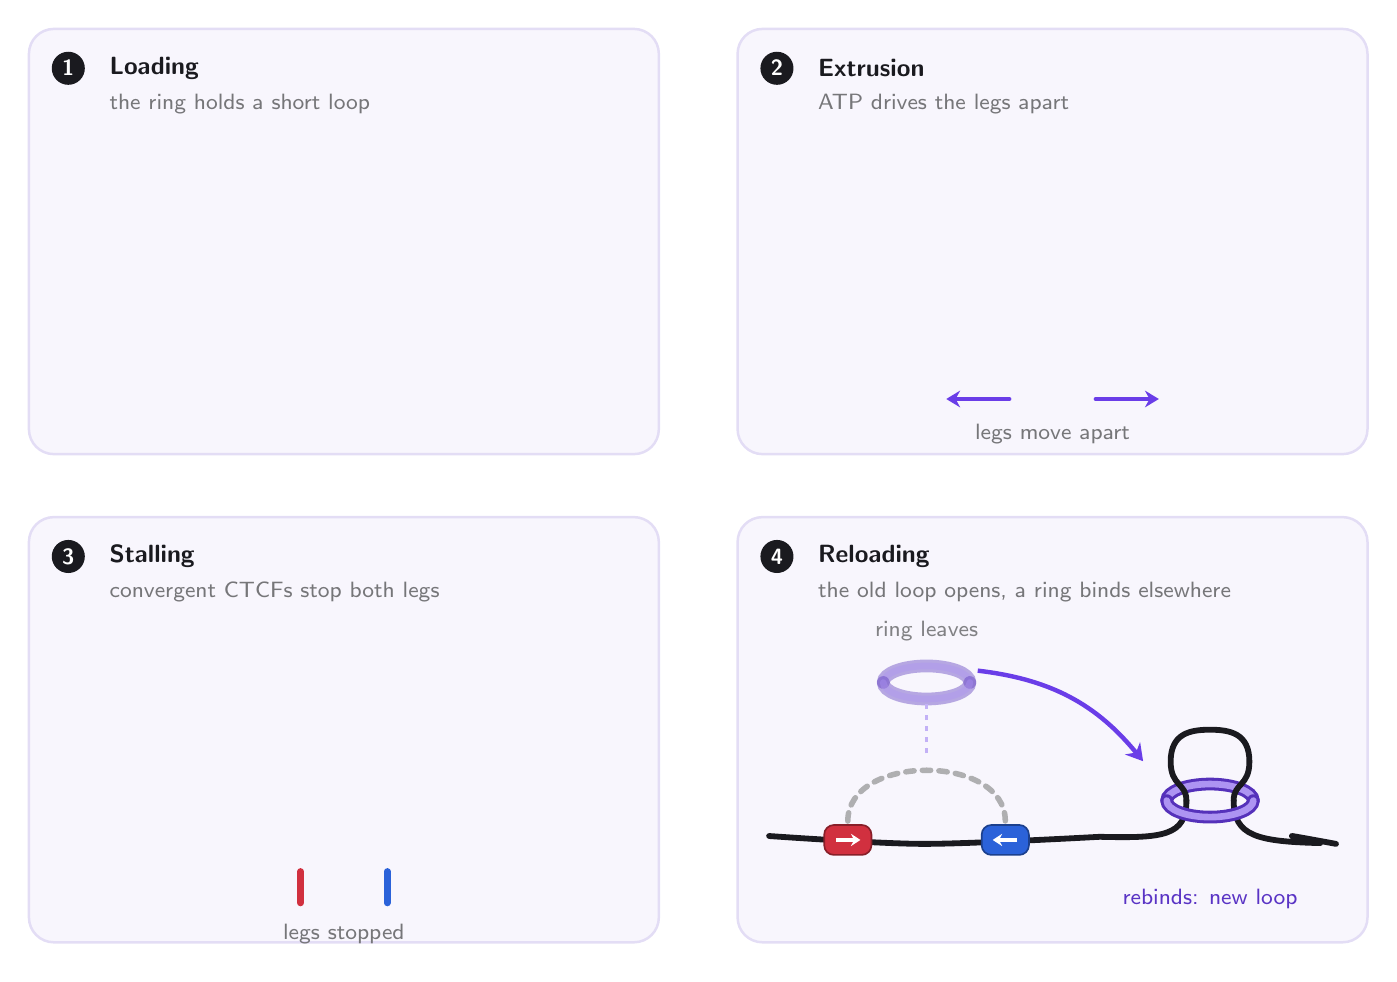
\begin{tikzpicture}
  \foreach \x/\y in {0/0,9/0,0/-6.2,9/-6.2}{\panelbg{\x}{\y-1.3}{\x+8}{\y+4.1}}
  \stage{0}{0}{0.6}{1.0}{2.9}
  \stage{9}{0}{0.95}{1.7}{1.9}
  \stage{0}{-6.2}{1.25}{2.2}{0.85}
  % panel 4: the ring leaves the fibre (old loop opens) and binds again elsewhere
  \begin{scope}[shift={(9,-6.2)}]
    \base{0.4}{7.6}{6.0}{0.5}
    \lloop{6.0}{0.5}{0.5}{0.9}{cohesin}
    \prot{1.4}{0}{f}\prot{3.4}{0}{r}
    % old loop opening (dashed) and the old ring lifting off the fibre
    \draw[line width=2pt,ink!35,dash pattern=on 3pt off 3pt,line cap=round] (1.4,0.24) .. controls (1.4,1.1) and (3.4,1.1) .. (3.4,0.24);
    \begin{scope}[opacity=0.4]\ringback{2.4}{2.0}{cohesin}\ringfront{2.4}{2.0}{cohesin}\end{scope}
    \draw[cohesin!40,line width=1.2pt,dash pattern=on 2pt off 2pt] (2.4,1.1)--(2.4,1.75);
    \draw[-{Stealth[length=6pt,width=7pt]},cohesin,line width=1.6pt] (3.05,2.15) to[bend left=22] (5.15,1.0);
    \node[note,text=ink!55] at (2.4,2.65) {ring leaves};
    \node[note,text=cohesin!85!black] at (6.0,-0.75) {rebinds: new loop};
  \end{scope}
  \badge{0.5}{3.6}{1}\badge{9.5}{3.6}{2}\badge{0.5}{-2.6}{3}\badge{9.5}{-2.6}{4}
  \node[hd] at (0.9,3.6) {Loading};\node[note,anchor=west] at (0.9,3.15) {the ring holds a short loop};
  \node[hd] at (9.9,3.6) {Extrusion};\node[note,anchor=west] at (9.9,3.15) {ATP drives the legs apart};
  \node[hd] at (0.9,-2.6) {Stalling};\node[note,anchor=west] at (0.9,-3.05) {convergent CTCFs stop both legs};
  \node[hd] at (9.9,-2.6) {Reloading};\node[note,anchor=west] at (9.9,-3.05) {the old loop opens, a ring binds elsewhere};
  % legs: moving (panel 2) and blocked (panel 3)
  \legarrow{12.45}{11.65}{-0.6}\legarrow{13.55}{14.35}{-0.6}
  \stopbar{3.45}{-6.2-0.6}{fwd}\stopbar{4.55}{-6.2-0.6}{rev}
  \node[note] at (4,-6.2-1.2) {legs stopped};
  \node[note] at (13,-1.05) {legs move apart};
\end{tikzpicture}
\end{document}
